% ============================================================
%  DINÁMICA DE SISTEMAS — LISTA DE ESPERA NO-GES
%  CIRUGÍA GENERAL — Servicio de Salud Valparaíso–San Antonio
%  Modelo de stock único, calibrado y validado (2021–2025)
% ============================================================
\documentclass[12pt,a4paper]{article}

% ── Encoding & Language ──────────────────────────────────────
\usepackage[utf8]{inputenc}
\usepackage[T1]{fontenc}
\usepackage[spanish,es-nodecimaldot]{babel}

% ── Layout ───────────────────────────────────────────────────
\usepackage[top=2.5cm,bottom=2.5cm,left=2.8cm,right=2.8cm]{geometry}
\usepackage{setspace}
\setstretch{1.15}
\usepackage{parskip}

% ── Math ─────────────────────────────────────────────────────
\usepackage{amsmath,amssymb,mathtools}

% ── Graphics & Diagrams ──────────────────────────────────────
\usepackage{graphicx}
\graphicspath{{resources/pictures/}}
\usepackage{tikz}
\usetikzlibrary{arrows.meta,positioning,shapes.geometric,
                decorations.pathmorphing,calc,fit,backgrounds,
                arrows,shapes.arrows,bending}
\usepackage{pgfplots}
\pgfplotsset{compat=1.18}

% ── Tables ───────────────────────────────────────────────────
\usepackage{booktabs,longtable,array,tabularx,multirow}
\usepackage{colortbl}
\usepackage{makecell}

% ── Colors ───────────────────────────────────────────────────
\usepackage[dvipsnames]{xcolor}
\definecolor{azulDS}{RGB}{0,74,124}
\definecolor{verdeDS}{RGB}{0,128,94}
\definecolor{rojoDS}{RGB}{180,40,40}
\definecolor{ambarDS}{RGB}{200,140,0}
\definecolor{grisClaro}{RGB}{245,245,245}
\definecolor{grisOscuro}{RGB}{80,80,80}

% ── Hyperlinks ───────────────────────────────────────────────
\usepackage[colorlinks=true,
            linkcolor=azulDS,
            citecolor=verdeDS,
            urlcolor=azulDS]{hyperref}
\usepackage{url}

% ── Captions & Floats ────────────────────────────────────────
\usepackage{caption,subcaption,float}
\captionsetup{labelfont=bf,font=small}

% ── Headers / Footers ────────────────────────────────────────
\usepackage{fancyhdr}
\pagestyle{fancy}
\fancyhf{}
\fancyfoot[C]{\thepage}
\renewcommand{\headrulewidth}{0pt}

% ── Boxes ────────────────────────────────────────────────────
\usepackage{tcolorbox}
\tcbuselibrary{skins,breakable}
\newtcolorbox{definicion}[1][]{
  colback=azulDS!5,colframe=azulDS!60,
  fonttitle=\bfseries,title=Definición,#1}
\newtcolorbox{arquetipobox}[2][]{
  colback=verdeDS!5,colframe=verdeDS!60,
  fonttitle=\bfseries,title=Arquetipo: #2,#1}
\newtcolorbox{databox}[1][]{
  colback=ambarDS!5,colframe=ambarDS!60,
  fonttitle=\bfseries,title=Fuentes de datos,#1}
\newtcolorbox{fasebox}[2][]{
  colback=azulDS!3,colframe=azulDS!50,
  fonttitle=\bfseries\large,title=#2,#1}

% ── Misc ─────────────────────────────────────────────────────
\usepackage{enumitem}
\usepackage{pifont}

% ============================================================
\begin{document}

% ── Portada ──────────────────────────────────────────────────
\begin{titlepage}
  \centering
  \vspace*{1cm}
  {\color{azulDS}\rule{\linewidth}{1.5pt}}\\[0.8em]
  {\LARGE\bfseries Dinámica de Sistemas:\\[0.3em]
    Lista de Espera No-GES de\\[0.3em]
    Cirugía General (SSVSA)}\\[0.6em]
  {\color{azulDS}\rule{\linewidth}{1.5pt}}

  \vspace{2cm}
  {\large Modelamiento Causal, Formulación, Validación\\
    e Implementación de Políticas sobre la Lista de Espera\\
    No-GES de Cirugía General del Hospital Eduardo Pereira}

  \vspace{3cm}
  \begin{tabular}{ll}
    \textbf{Caso:}        & Cirugía General No-GES — Hospital Eduardo Pereira (CDE) \\[4pt]
    \textbf{Servicio:}    & Servicio de Salud Valparaíso--San Antonio (SSVSA)       \\[4pt]
    \textbf{Integrantes:} & Eric Escudero, Pitehr Hurtado                           \\[4pt]
    \textbf{Fecha:}       & \today                                                  \\[4pt]
  \end{tabular}

\end{titlepage}

\tableofcontents
\newpage

% ============================================================
\section{Introducción}
% ============================================================

Las listas de espera quirúrgicas No-GES constituyen uno de los problemas de equidad y eficiencia más persistentes del sistema de salud público chileno. A diferencia de las patologías cubiertas por las Garantías Explícitas en Salud (GES), que establecen plazos máximos de atención con respaldo legal, las prestaciones No-GES carecen de garantía de oportunidad vinculante, lo que las expone de manera crónica a un desequilibrio entre la demanda generada por la red asistencial y la capacidad resolutiva del sector público. Este desequilibrio no es estático: genera dinámicas de retroalimentación que se auto-refuerzan, haciendo que las intervenciones puntuales sobre los síntomas ---ampliación transitoria de horas, resolución de casos de mayor antigüedad--- sean insuficientes para revertir la tendencia estructural.

El caso de Cirugía General del Hospital Eduardo Pereira (CDE), dependiente del Servicio de Salud Valparaíso--San Antonio (SSVSA), es ilustrativo de esta dinámica. Entre enero de 2021 y julio de 2025 la lista de espera No-GES creció de 683 a 2\,202 pacientes, un incremento acumulado del 222\,\% en 55 meses, equivalente a una tasa media de $\approx 27$ pacientes adicionales por mes. Este crecimiento es sostenido, monótono y cualitativamente robusto frente a variaciones en la entrada de derivaciones, lo que sugiere que su causa raíz no reside en perturbaciones exógenas sino en la arquitectura de retroalimentación del propio sistema.

La modelación matemática de este tipo de fenómenos requiere un marco que represente explícitamente los mecanismos causales y los bucles de retroalimentación, no solo las correlaciones históricas. La Dinámica de Sistemas (DS) provee ese marco: parte del principio de que el comportamiento es consecuencia de la estructura, y propone que la intervención más efectiva es aquella que modifica la estructura y no el síntoma (Sterman, 2000~\ref{ref:sterman}; Meadows, 2008~\ref{ref:meadows}). Su aplicación a sistemas de salud y listas de espera tiene amplio respaldo en la literatura internacional (González-Busto y García, 1999~\ref{ref:gonzalez}; Wolstenholme, 1999~\ref{ref:wolstenholme}; Brailsford \textit{et al.}, 2004~\ref{ref:brailsford}; Homer y Hirsch, 2006~\ref{ref:homer}), y el presente trabajo constituye una aplicación sistemática a una lista de espera No-GES del sistema público chileno.

El modelo identifica la estructura de retroalimentación que genera el crecimiento observado, la cuantifica mediante parámetros calibrados sobre datos SIGTE y evalúa el efecto diferencial de intervenciones de política bajo incertidumbre estocástica. Las contribuciones principales son: (i) un modelo de DS calibrado y validado formalmente para una lista de espera No-GES del sistema público chileno; (ii) la identificación y cuantificación del punto de inflexión estructural del sistema; (iii) la endogenización del mecanismo de erosión de capacidad como proceso irreversible; y (iv) la evaluación de escenarios de política con análisis de sensibilidad y banda de incertidumbre Monte Carlo.

El documento se organiza en cuatro fases metodológicas: la \textbf{Fase 1} establece el propósito, los límites del sistema, los modos de referencia y la hipótesis dinámica; la \textbf{Fase 2} desarrolla la formulación matemática completa y la parametrización; la \textbf{Fase 3} ejecuta la batería de validación de Barlas (1989)~\ref{ref:barlas}; y la \textbf{Fase 4} evalúa tres escenarios de política en modo estocástico y extrae las implicancias sistémicas para la gestión del SSVSA.

% ============================================================
\section{Fase 1: Conceptualización}
% ============================================================

\subsection{Propósito del Modelo}

\subsubsection*{Antecedentes y Revisión de Literatura}

La modelación de listas de espera mediante Dinámica de Sistemas cuenta con una tradición consolidada. González-Busto y García (1999)~\ref{ref:gonzalez} analizaron las listas quirúrgicas del sistema público español e identificaron el mismo patrón de crecimiento sostenido bajo desequilibrio estructural entre flujos de entrada y salida, concluyendo que las políticas de choque sobre la demanda son inefectivas en ausencia de reformas a la capacidad. Wolstenholme (1999)~\ref{ref:wolstenholme} extendió este marco al National Health Service (NHS) del Reino Unido, mostrando cómo la fuga al sector privado actúa como válvula de escape que estabiliza la lista a un nivel elevado pero no la reduce. Brailsford \textit{et al.} (2004)~\ref{ref:brailsford} sistematizaron el uso de la DS en servicios de urgencias, identificando el mismo arquetipo de \textit{Limits to Growth} con bucles balanceadores insuficientes. Homer y Hirsch (2006)~\ref{ref:homer} argumentaron que la DS es la metodología más adecuada para intervenciones de política en salud pública cuando el problema exhibe retroalimentación, retardos y no-linealidades ---características todas presentes en el sistema bajo estudio.

En el contexto chileno, la literatura sobre listas de espera No-GES es escasa desde la perspectiva de la modelación formal. Los reportes del DEIS/MINSAL documentan el fenómeno en términos estadísticos pero no analizan su estructura causal. El presente trabajo busca llenar esa brecha mediante una aplicación sistemática de la DS a una lista de espera No-GES de Cirugía General en el sistema público chileno.

\subsubsection*{Definición del Problema}

El problema central es un desequilibrio estructural entre flujos: la tasa de ingreso de derivaciones ($E \approx 275$ pac/mes) supera de forma persistente la capacidad resolutiva pública ($C \approx 240$ pac/mes), generando un flujo neto positivo de $\approx 35$ pac/mes que no puede ser absorbido completamente por los mecanismos de alivio existentes (fuga al privado y egresos administrativos). El problema se agrava por un mecanismo endógeno de erosión: cuando la lista crece, el tiempo de espera aumenta; cuando la fuga al privado supera su máximo histórico, el especialista migra horas del sector público al privado de manera irreversible, reduciendo la capacidad pública y amplificando la brecha. Este mecanismo de \textit{Deadly Spiral} convierte un desequilibrio de flujos en un proceso acumulativo auto-reforzado.

\subsubsection*{Pregunta de Investigación}

\begin{tcolorbox}[colback=azulDS!5,colframe=azulDS!60]
  \textbf{Pregunta principal:} ¿Qué factores estructurales explican el crecimiento persistente de la lista de espera No-GES de Cirugía General del SSVSA entre 2021 y 2025, y qué política permite estabilizar o revertir esa tendencia?

  \medskip
  \textbf{Sub-preguntas operacionales:}
  \begin{enumerate}[leftmargin=1.2cm,label=(\roman*)]
    \item ¿Cuál es la contribución relativa de cada bucle de retroalimentación al comportamiento observado?
    \item ¿En qué punto de la dotación de especialistas el sistema cruza el umbral de estabilización (\textit{tipping point})?
    \item ¿Qué combinación de políticas minimiza la lista en el horizonte 2021--2025 bajo incertidumbre estocástica?
  \end{enumerate}
\end{tcolorbox}

\subsubsection*{Usuarios Potenciales del Modelo}

\begin{itemize}[leftmargin=1.5cm]
  \item \textbf{Dirección del SSVSA} — gestión de redes asistenciales: evaluación cuantitativa del efecto de aumentos en la dotación de especialistas de Cirugía General sobre la trayectoria de la lista.
  \item \textbf{Jefatura del Servicio de Cirugía} del Hospital Eduardo Pereira: planificación de capacidad, horas resolutivas y política de retención de especialistas.
  \item \textbf{Unidad de gestión de la demanda (SIGTE)}: priorización, depuración activa y monitoreo de la lista bajo distintos supuestos de egreso administrativo.
  \item \textbf{Autoridades sanitarias regionales y nacionales}: diseño de políticas de reducción de listas No-GES replicables en otros servicios de salud con estructura similar.
  \item \textbf{Investigadores} en gestión sanitaria, dinámica de sistemas y política pública de salud.
\end{itemize}

\subsubsection*{Objetivo del Modelo}

El objetivo principal es reproducir la dinámica histórica de crecimiento de la lista de espera No-GES de Cirugía General entre enero de 2021 y julio de 2025, identificar la estructura causal que genera ese crecimiento y evaluar el efecto diferencial de tres políticas alternativas: (i) aumento de la dotación de especialistas en el sector público, (ii) depuración activa de la lista mediante egresos administrativos, y (iii) retención de especialistas mediante la mitigación del diferencial salarial que activa el bucle de erosión de capacidad.

El modelo no busca predecir la trayectoria futura de la lista sino demostrar que la estructura identificada es suficiente para reproducir el comportamiento observado y que las políticas evaluadas producen efectos cualitativamente distintos sobre esa estructura.

\subsubsection*{Periodo de Simulación y Resolución Temporal}

\begin{itemize}[leftmargin=1.5cm]
  \item \textbf{Horizonte:} 55 meses, desde enero 2021 a julio 2025. El modelo \emph{no proyecta a futuro}: se simula sobre la ventana histórica para validar la estructura contra lo observado.
  \item \textbf{Resolución temporal:} datos de SIGTE por mes.
  \item \textbf{Paso de integración:} $DT = 1/32 = 0.03125$ mes.
  \item \textbf{Método numérico:} Euler. Para un modelo con no-linealidades suaves y escalón mensual de capacidad, Euler con un $DT$ pequeño es suficiente; la elección se verifica en la Fase 3 mediante el test de error de integración (Barlas, 1989~\ref{ref:barlas}).
\end{itemize}

\subsection{Límites del Sistema — Clasificación de Variables}

Se identifican las variables relevantes que explican el comportamiento de interés, clasificándolas según su posición en los límites del modelo y su función en la dinámica de sistemas. El stock central es el número de pacientes en lista, no el tiempo de espera; este último es una variable derivada por la Ley de Little (Sterman, 2000~\ref{ref:sterman}; Little, 1961~\ref{ref:little}).

\begin{table}[H]
  \centering
  \caption{Clasificación de variables del modelo}
  \label{tab:variables}
  \begin{tabularx}{\textwidth}{@{}p{5.6cm}cccccc@{}}
    \toprule
    \rowcolor{azulDS!15}
    \multirow{2}{*}{\textbf{Variable}}              &
    \multicolumn{2}{c}{\textbf{Límites del modelo}} &
    \multicolumn{3}{c}{\textbf{Función en DS}}                                                                                               \\
    \cmidrule(lr){2-3}\cmidrule(lr){4-6}
    \rowcolor{azulDS!8}
                                                    & \textbf{Endóg.} & \textbf{Exóg.} & \textbf{Nivel} & \textbf{Flujo} & \textbf{Auxiliar} \\
    \midrule
    Lista de espera CG $L(t)$                       & \checkmark      &                & \checkmark     &                &                   \\
    Entrada (derivaciones)                          &                 & \checkmark     &                & \checkmark     &                   \\
    Atención (resolución pública)                   & \checkmark      &                &                & \checkmark     &                   \\
    Fuga al privado                                 & \checkmark      &                &                & \checkmark     &                   \\
    Egreso varios (administrativo)                  & \checkmark      &                &                & \checkmark     &                   \\
    Tiempo de espera                                & \checkmark      &                &                &                & \checkmark        \\
    Capacidad de atención                           & \checkmark      &                &                &                & \checkmark        \\
    Horas públicas $H_{\text{pub}}(t)$              & \checkmark      &                &                &                & \checkmark        \\
    Horas migradas acumuladas                       & \checkmark      &                & \checkmark     &                &                   \\
    $\mu$ de fuga (media NB)                        & \checkmark      &                &                &                & \checkmark        \\
    \midrule
    Horas totales por especialista                  &                 & \checkmark     &                &                &                   \\
    Ratio público / atención                        &                 & \checkmark     &                &                &                   \\
    Pacientes por hora                              &                 & \checkmark     &                &                &                   \\
    N.º de especialistas                            &                 & \checkmark     &                &                &                   \\
    Tasa egreso varios                              &                 & \checkmark     &                &                &                   \\
    Sensibilidad a la brecha                        &                 & \checkmark     &                &                &                   \\
    Coeficientes NB ($\beta_0,\beta_1,\theta$)      &                 & \checkmark     &                &                &                   \\
    \bottomrule
  \end{tabularx}
\end{table}

\subsubsection*{Justificación de los límites}

\textbf{Variables endógenas.} El stock central $L(t)$ y los tres flujos de salida (atención, fuga, egreso) son endógenos porque sus valores en cada período son determinados por la estructura del modelo. Las horas públicas $H_{\text{pub}}(t)$ y las horas migradas acumuladas $H_{\text{migr}}(t)$ se incluyen como endógenas porque forman parte del bucle de erosión R1: su dinámica retroalimenta la capacidad y, por esa vía, la lista.

\textbf{Entrada como variable exógena.} La tasa de derivaciones es exógena porque su generación ocurre fuera del límite del modelo: proviene de la Atención Primaria de Salud (APS), de las interconsultas de otras especialidades y de los protocolos de referencia del SSVSA, ninguno de los cuales es controlado por el Servicio de Cirugía del CDE. Incluir la dinámica de la APS requeriría un modelo de mayor escala que va más allá del propósito declarado.

\textbf{Parámetros de capacidad como exógenos.} Las horas contratadas por especialista ($h_{\text{tot}}$), los ratios de dedicación ($r_{\text{pub}}, r_{\text{at}}$) y la productividad ($p_h$) se tratan como parámetros fijos porque su variación depende de decisiones administrativas y contractuales que no responden de forma continua al estado de la lista. Son, en el sentido de Sterman (2000)~\ref{ref:sterman}, variables de política evaluadas en los escenarios de la Fase 4.

\subsubsection*{Variables excluidas y justificación}

Las siguientes variables relevantes fueron explícitamente dejadas fuera del modelo:

\begin{itemize}[leftmargin=1.5cm]
  \item \textbf{Estacionalidad de las derivaciones.} Los datos SIGTE muestran variabilidad mensual ($\sigma_E = 60.16$ pac/mes) sin un patrón estacional sistemático identificable en 55 meses. El modo normal captura esta variabilidad mediante distribución Normal calibrada.
  \item \textbf{Heterogeneidad por prioridad o complejidad.} El modelo trata a todos los pacientes en lista como homogéneos. Una desagregación por prioridad (urgente, menos urgente, electivo) requeriría stocks separados y datos de distribución por categoría que no están disponibles en SIGTE a nivel de serie mensual.
  \item \textbf{Capacidad del sector privado.} Se supone que el sector privado tiene capacidad suficiente para absorber toda la fuga modelada. Esta es una aproximación razonable en el horizonte de 55 meses estudiado, pero podría ser un límite en horizontes más largos o ante aumentos muy grandes de la fuga.
  \item \textbf{Incentivos al retorno desde el privado.} Una vez que un paciente fuga al privado, se supone que no retorna a la lista pública. Esta simplificación es consistente con la naturaleza irreversible de la resolución quirúrgica privada.
\end{itemize}

\subsection{Modos de Referencia}

\subsubsection*{Comportamiento Histórico}

El modo de referencia se construye a partir de la serie mensual de la lista de espera No-GES de Cirugía General registrada en el Sistema de Información para la Gestión de Tiempos de Espera (SIGTE) del SSVSA, correspondiente a 55 observaciones mensuales entre enero de 2021 y julio de 2025. La serie exhibe un crecimiento sostenido, monotónico y sin reversiones, con una pendiente media de $\approx 27$ pacientes adicionales por mes. El Cuadro~\ref{tab:historico} presenta los hitos clave de la serie y su interpretación en términos del modelo.

\begin{table}[H]
  \centering
  \caption{Comportamiento histórico — Lista de espera No-GES de Cirugía General, SSVSA (hitos anuales)}
  \label{tab:historico}
  \begin{tabular}{@{}lrrp{5.8cm}@{}}
    \toprule
    \rowcolor{azulDS!15}
    \textbf{Fecha} & \textbf{Lista (pac.)} & \textbf{$\Delta$ anual} & \textbf{Observación}                                          \\
    \midrule
    2021-01        & 683                   & ---                     & Condición inicial $L_0$; inicio de la ventana de simulación   \\[2pt]
    2022-01        & 993                   & +310                    & Primer año completo; tasa de crecimiento $\approx 26$ pac/mes \\[2pt]
    2023-01        & 1305                  & +312                    & Crecimiento sostenido; brecha capacidad--demanda persiste     \\[2pt]
    2024-01        & 1622                  & +317                    & Pendiente estable; ausencia de reversión                      \\[2pt]
    2025-01        & 1940                  & +318                    & Cuarto año; sistema aún sin punto de inflexión                \\[2pt]
    2025-07        & 2202                  & +262                    & Observación final (6 meses); $+222$\,\% respecto a $L_0$      \\
    \bottomrule
    \multicolumn{4}{l}{\footnotesize Fuente: SIGTE-SSVSA, serie mensual de Cirugía General (55 meses, ene-2021 a jul-2025).}         \\
    \multicolumn{4}{l}{\footnotesize Valores intermedios 2022--2025 estimados por interpolación lineal sobre la serie calibrada.}
  \end{tabular}
\end{table}

\begin{databox}
  \textbf{Fuente primaria:} SIGTE-SSVSA — Sistema de Información para la Gestión de Tiempos de Espera, Servicio de Salud Valparaíso--San Antonio. Serie mensual de Cirugía General No-GES, Hospital Eduardo Pereira (CDE). Período: enero 2021 -- julio 2025 (55 registros). Los datos incluyen: lista de espera por mes, entrada de derivaciones por mes y egresos por categoría (atención, fuga al privado, egreso administrativo).
\end{databox}

\subsubsection*{Caracterización estadística de la serie de derivaciones}

La serie de entrada (derivaciones mensuales al servicio de Cirugía General) presenta las siguientes propiedades estadísticas, relevantes para la calibración del modo normal:

\begin{itemize}[leftmargin=1.5cm]
  \item \textbf{Media:} $\bar{E} = 274.6$ pac/mes
  \item \textbf{Desviación estándar:} $\sigma_E = 60.16$ pac/mes (coeficiente de variación $\approx 21.9$\,\%)
  \item \textbf{Rango observado:} mín.\ $\approx 150$ pac/mes, máx.\ $\approx 420$ pac/mes
  \item \textbf{Patrón temporal:} no se identifica estacionalidad sistemática en la ventana de 55 meses; la variabilidad es cuasi-aleatoria en torno a la media, lo que justifica el modelo de entrada Normal i.i.d.
\end{itemize}

La brecha estructural entre la media de entrada ($274.6$ pac/mes) y la capacidad base ($C_0 = 240$ pac/mes) es de $\approx 34.6$ pac/mes, valor que ---en ausencia de intervención--- genera el crecimiento monotónico observado. Esta brecha es el motor primario del comportamiento de referencia.

\subsubsection*{Modos de Entrada: Histórico y Normal}

El modelo admite dos modos de entrada sobre la misma ventana de 55 meses:

\begin{itemize}[leftmargin=1.5cm]
  \item \textbf{Modo histórico:} la entrada es la serie real de derivaciones de Cirugía General (55 valores mensuales embebidos). Se usa de forma determinista para reproducir exactamente la trayectoria observada.
  \item \textbf{Modo normal (Monte Carlo):} la entrada se sortea como $\text{Entrada}_t \sim \mathcal{N}(\mu=274.6,\ \sigma=60.16)$ pacientes/mes, calibrada sobre la misma ventana. Incorpora la aleatoriedad realista de las derivaciones y, combinada con el sorteo estocástico de la fuga, produce una banda de incertidumbre.
\end{itemize}

\begin{definicion}
  Todos los análisis cuantitativos de este informe (validación de comportamiento, sensibilidad y escenarios de política) se ejecutan en \textbf{modo normal} con 200 réplicas Monte Carlo, reportando la media y la banda de percentiles 5--95\%. El modo histórico se usa únicamente como trayectoria de referencia determinista.
\end{definicion}

\subsubsection*{Modo de Comportamiento Esperado}

El sistema exhibe un crecimiento sostenido al alza, característico de un sistema donde la tasa de ingreso supera crónicamente la tasa de egreso. Los bucles balanceadores (fuga al privado y egresos administrativos) frenan el crecimiento pero son insuficientes para revertirlo en ausencia de intervención sobre la capacidad. El arquetipo dominante es \textit{Límites al Crecimiento}, acoplado con una de erosión de capacidad (sección~\ref{sec:arquetipos}).

La Figura 1 muestra la banda Monte Carlo del modo normal, la trayectoria del modo histórico y el punto observado de julio de 2025.

\begin{figure}[H]
  \centering
  \includegraphics[width=1\linewidth]{fig5_modos_referencia.png}
  \caption{Modo de referencia: banda Monte Carlo del modo normal (5--95\%, 200 réplicas),
    trayectoria del modo histórico (entradas reales) y punto observado en julio de 2025
    ($L=2202$). El observado cae dentro de la banda de incertidumbre.}
  \label{fig:modos_referencia}
\end{figure}
\subsection{Ciclos de Retroalimentación — Hipótesis Dinámica}
\label{sec:arquetipos}

El modelo identifica tres bucles de retroalimentación que gobiernan la dinámica observada: dos bucles balanceadores ---la fuga de pacientes al sector privado (B1), cuya intensidad crece de forma exponencial con el tiempo de espera, y el drenaje administrativo de la lista (B2)--- y un bucle reforzador endógeno de erosión de capacidad (R1), denominado \textit{Deadly Spiral}: cuando la fuga supera su máximo histórico, el especialista migra horas del sector público al privado de manera irreversible, deteriorando la capacidad pública y amplificando el crecimiento de la lista.

\subsubsection*{Descripción de los Bucles}

\begin{description}[leftmargin=1cm,style=nextline]
  \item[\textcolor{verdeDS}{\textbf{B1 — Balance: Fuga al Sector Privado}}]
        A medida que la lista crece, el tiempo de espera aumenta. Ante esperas más largas, una fracción creciente de pacientes migra al sector privado, drenando la lista pública. La relación no es lineal sino exponencial: la fuga se modela con una regresión Binomial Negativa cuya media crece exponencialmente con la mediana del tiempo de espera. Este bucle actúa como una válvula de escape (González-Busto y García, 1999~\ref{ref:gonzalez}; Wolstenholme, 1999~\ref{ref:wolstenholme}).\\
        Cadena: $L(t) \overset{+}{\to} T_{\text{esp}} \overset{+}{\to} \text{Fuga} \overset{-}{\to} L(t)$ \quad\textbf{BALANCE}

  \item[\textcolor{verdeDS}{\textbf{B2 — Balance: Drenaje Administrativo}}]
        La lista genera salidas administrativas constantes (fallecidos en espera, desistimientos, duplicados, cambios de previsión) que no migran al privado.\\
        Cadena: $L(t) \overset{+}{\to} E_{\text{adm}} \overset{-}{\to} L(t)$ \quad\textbf{BALANCE}

  \item[\textcolor{rojoDS}{\textbf{R1 — Refuerzo: Espiral de Erosión de Capacidad (Deadly Spiral)}}]
        Cuando la fuga al privado supera su máximo histórico, el especialista construye capacidad privada permanente migrando horas del sector público al privado. Menos horas públicas reducen la capacidad de atención, lo que alarga la espera, aumenta la fuga y puede gatillar un nuevo récord. A diferencia de la revisión bibliográfica este bucle es \emph{endógeno}.\\
        Cadena: $L(t) \overset{+}{\to} T_{\text{esp}} \overset{+}{\to} \text{Fuga} \overset{+}{\to} H_{\text{migr}} \overset{-}{\to} H_{\text{pub}} \overset{+}{\to} \text{Capacidad} \overset{-}{\to} L(t)$ \quad\textbf{REFUERZO}
\end{description}

\begin{tcolorbox}[colback=rojoDS!5,colframe=rojoDS!60,fonttitle=\bfseries,
    title=Lógica de récord del bucle R1]
  La migración de horas es irreversible: $H_{\text{migr}}$ solo crece. Por eso únicamente un \emph{nuevo} máximo de fuga ($\Delta = \max(\text{fuga} - \text{fuga}_{\max},\,0) > 0$) justifica migrar horas adicionales. Si la fuga baja y vuelve a subir al mismo nivel previo, el especialista ya tiene esa capacidad privada construida y no migra más. El parámetro \texttt{sensibilidad\_brecha} $\in[0,1]$ modula cuánto le importa la brecha salarial al especialista.
\end{tcolorbox}

\subsubsection*{Arquetipos Sistémicos}

Los bucles identificados dan lugar a dos arquetipos de comportamiento reconocidos en la literatura de DS (Senge, 1990~\ref{ref:senge}; Wolstenholme, 2004~\ref{ref:wolstenholme}):

\begin{arquetipobox}{Límites al Crecimiento (\textit{Limits to Growth})}
  El stock $L(t)$ crece impulsado por la brecha $E > C$, pero los bucles balanceadores B1 (fuga exponencial) y B2 (drenaje administrativo) actúan como frenos. En el rango de la lista observado (683--2202 pac.), B1 y B2 son insuficientes para compensar la brecha, pero a listas muy altas ($L \gg 5000$ pac.) la fuga NB explotaría y vaciaría el sistema. El arquetipo predice que intervenciones sobre los síntomas (aumentar la capacidad puntualmente) sin atacar la brecha estructural solo retardan el crecimiento.
\end{arquetipobox}

\begin{arquetipobox}{Erosión de Metas (\textit{Eroding Goals} / \textit{Deadly Spiral})}
  El bucle R1 endogeniza el deterioro de la capacidad: cuando la lista crece, la fuga aumenta; cuando la fuga supera su récord, el especialista migra horas de forma irreversible. Esto reduce la capacidad pública, amplifica la brecha y acelera el crecimiento futuro de la lista. La irreversibilidad de $H_{\text{migr}}$ convierte este arquetipo en un ratchet: una vez activado, solo puede contrarrestarse aumentando la capacidad total (nuevo especialista) o eliminando el incentivo salarial ($s_{\text{brecha}} = 0$).
\end{arquetipobox}

\subsubsection*{Análisis de dominancia de bucles}

La dominancia de cada bucle varía con el nivel de la lista:

\begin{itemize}[leftmargin=1.5cm]
  \item \textbf{Lista baja} ($L < 500$ pac.): la fuga NB es pequeña ($\mu \approx 2$--$3$ pac/mes) y el egreso administrativo ($g = 7$ pac/mes) es comparable a la fuga. Domina el motor de crecimiento ($E - C > 0$); B1 y B2 son marginales.
  \item \textbf{Lista media} ($500 < L < 2000$ pac.): $T_{\text{esp}}$ crece, $\mu_{\text{NB}}$ aumenta exponencialmente. B1 cobra fuerza pero sigue siendo insuficiente. R1 puede activarse si la fuga supera su récord histórico.
  \item \textbf{Lista alta} ($L > 2000$ pac.): la fuga exponencial se convierte en el mecanismo dominante; en el límite extremo ($C \to 0$), B1 vacía la lista por sí solo (confirmado en la Prueba 2 de la Fase 3).
\end{itemize}

\subsubsection*{Diagrama Causal}

\begin{figure}[H]
  \centering
  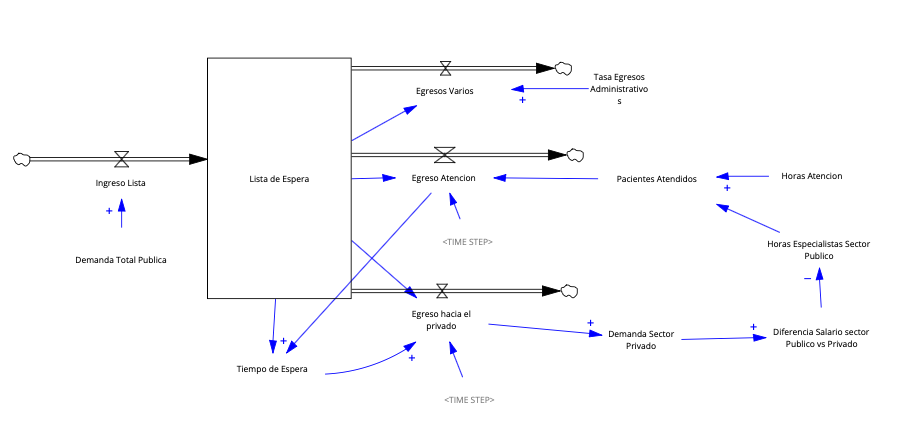
\includegraphics[width=1\linewidth]{diagrama de flujo.png}
  \caption{Diagrama causal del sistema de lista de espera No-GES de Cirugía General, SSVSA. Los bucles B1 y B2 son balanceadores; el bucle R1 es reforzador.}
  \label{fig:causal}
\end{figure}

\subsubsection*{Diagrama de Stocks y Flujos}

\begin{figure}[H]
  \centering
  \begin{tikzpicture}[
      stock/.style = {rectangle, minimum width=2.8cm, minimum height=1.1cm,
          draw=azulDS, fill=azulDS!10, thick, align=center, font=\small\bfseries},
      flow/.style  = {-{Stealth[length=9pt]}, ultra thick, color=azulDS!70},
      cloud/.style = {ellipse, minimum width=1.3cm, minimum height=0.75cm,
          draw=gray!50, fill=gray!8, font=\scriptsize, align=center},
      aux/.style   = {circle, minimum size=0.85cm,
          draw=verdeDS!70, fill=verdeDS!8, font=\scriptsize, align=center},
      param/.style = {diamond, minimum width=1.4cm, minimum height=0.7cm,
          draw=ambarDS!80, fill=ambarDS!8, font=\scriptsize, align=center},
      info/.style  = {-{Stealth[length=5pt]}, dashed, color=grisOscuro, thin},
      every node/.style={align=center},
    ]
    % ── Stock central ────────────────────────────────────────────
    \node[cloud]  (src)  at (-4.0,0) {};
    \node[stock]  (L)    at (0,0)   {$L(t)$\\Lista CG};
    \node[cloud]  (snk1) at (4.0,0.9) {};
    \node[cloud]  (snk2) at (4.0,-0.9){};
    \node[cloud]  (snk3) at (4.0,-2.4){};

    % ── Flujos ───────────────────────────────────────────────────
    \draw[flow] (src)   -- node[above,font=\scriptsize]{Entrada} (L);
    \draw[flow] (L)     -- node[above,font=\scriptsize,sloped]{Atención} (snk1);
    \draw[flow] (L)     -- node[below,font=\scriptsize,sloped]{Fuga} (snk2);
    \draw[flow] (L)     -- node[below,font=\scriptsize,sloped]{Egreso var.} (snk3);

    % ── Stock secundario: horas migradas ─────────────────────────
    \node[stock,fill=rojoDS!10,draw=rojoDS] (Hm) at (0,3.0) {$H_{\text{migr}}(t)$\\Horas migradas};
    \node[cloud] (srcH) at (-4.0,3.0) {};
    \draw[flow,color=rojoDS!70] (srcH) -- node[above,font=\scriptsize]{Migración\\(récord fuga)} (Hm);

    % ── Auxiliares ───────────────────────────────────────────────
    \node[aux]   (T)   at (0,-3.0)  {$T_{\text{esp}}$};
    \node[aux]   (fp)  at (2.4,-3.0){$\mu$ fuga};
    \node[aux]   (Hp)  at (-2.4,1.5){$H_{\text{pub}}$};
    \node[aux]   (Cap) at (-2.4,-1.5){Cap.};

    % ── Parámetros ───────────────────────────────────────────────
    \node[param] (nesp) at (-5.6, 0.9) {$n_{\text{esp}}$};
    \node[param] (NB)   at (4.6,-4.0)  {$\beta_0,\beta_1,\theta$};
    \node[param] (sens) at (3.2, 3.0)  {$s_{\text{brecha}}$};
    \node[param] (eg)   at (6.6,-2.4)  {$\tau_{\text{adm}}$};

    % ── Vínculos info ────────────────────────────────────────────
    \draw[info] (L)  -- (T);
    \draw[info] (T)  -- (fp);
    \draw[info] (fp) to[bend left=10] (snk2);
    \draw[info] (NB) -- (fp);
    \draw[info] (fp) to[bend right=30] (Hm);
    \draw[info] (sens) -- (Hm);
    \draw[info] (Hm) -- (Hp);
    \draw[info] (nesp) to[bend left=15] (Hp);
    \draw[info] (Hp) -- (Cap);
    \draw[info] (Cap) to[bend left=50] (snk1);
    \draw[info] (eg) to[bend left=10] (snk3);

  \end{tikzpicture}
  \caption{Diagrama de stocks y flujos. El rectángulo azul es el stock central $L(t)$;
    el rectángulo rojo es el stock acumulador $H_{\text{migr}}(t)$ (horas migradas,
    monótono creciente). Las nubes son fuentes/sumideros; los círculos son auxiliares;
    los diamantes son parámetros. Las flechas discontinuas son vínculos de información.}
  \label{fig:stocks}
\end{figure}

% ============================================================
\section{Fase 2: Formulación}
% ============================================================

\subsection{Estructura del Modelo}

El modelo se implementa en Python. Tiene \textbf{1 stock central} ($L$), \textbf{1 stock acumulador} ($H_{\text{migr}}$), \textbf{1 flujo de entrada} y \textbf{3 flujos de salida} (atención, fuga, egreso varios), más las variables auxiliares de capacidad, tiempo de espera y media de la fuga.

\begin{definicion}
  \textbf{Consistencia dimensional:} el stock $L(t)$ tiene unidades de \textit{pacientes}. Los flujos son \textit{pacientes/mes}. El tiempo de espera es \textit{meses} (o \textit{días} para el predictor de la fuga). La capacidad es \textit{pacientes/mes}, producto de \textit{horas/mes}, \textit{pacientes/hora} y fracciones adimensionales. El stock $H_{\text{migr}}$ está en \textit{horas/mes}.
\end{definicion}

\subsection{Formulación Matemática}

\subsubsection*{Variable de Nivel (Stock Central)}

El nivel central es la lista de espera $L(t)$, expresada como ecuación integral:

\begin{equation}
  \boxed{
    L(t) = L_0 + \int_0^t \left[ E(\tau) - A(\tau) - F(\tau) - G(\tau) \right] d\tau
  }
  \label{eq:nivel}
\end{equation}

con $L(0) = L_0 = 683$ pacientes (enero 2021), donde $E$ es la entrada, $A$ la atención, $F$ la fuga al privado y $G$ el egreso varios. En forma diferencial:

\begin{equation}
  \frac{dL}{dt} = E(t) - A(t) - F(t) - G(t)
\end{equation}

\subsubsection*{Flujos de Salida con Acotamiento}

Todo flujo de salida se acota con un $\min$ respecto a lo disponible en el stock, garantizando que $L$ nunca sea negativo (Sterman, 2000~\ref{ref:sterman}):

\begin{align}
  A(t) & = \min\!\left( C(t),\ \tfrac{L(t)}{DT} \right) \quad [\text{pac/mes}] \label{eq:atencion}                                      \\[4pt]
  F(t) & = \min\!\left( F_{\text{NB}}(t),\ \max\!\bigl(\tfrac{L(t)}{DT} - A(t),\,0\bigr) \right) \quad [\text{pac/mes}] \label{eq:fuga} \\[4pt]
  G(t) & = \min\!\left( g,\ \max\!\bigl(\tfrac{L(t)}{DT} - A(t) - F(t),\,0\bigr) \right) \quad [\text{pac/mes}] \label{eq:egreso}
\end{align}

con $g = 7$ pac/mes (egreso varios administrativo: fallecidos, desistimientos que no van al privado, duplicados, cambios de previsión).

\subsubsection*{Capacidad de Atención (desagregada)}

La capacidad resolutiva del sector público se desagrega como el producto de horas, fracciones de dedicación y productividad:

\begin{equation}
  C(t) = H_{\text{pub}}(t)\cdot r_{\text{at}}\cdot p_h
  \label{eq:capacidad}
\end{equation}

donde $H_{\text{pub}}(t)$ son las horas públicas vigentes, $r_{\text{at}}=0.30$ es la fracción de horas públicas dedicadas a atender la lista y $p_h=2.0$ pac/hora la productividad. Las horas públicas base se construyen a partir de la dotación:

\begin{equation}
  H_{\text{pub}}^{\,0} = h_{\text{tot}}\cdot r_{\text{pub}}\cdot n_{\text{esp}}
  = 160 \times 0.50 \times 5.0 = 400 \ \text{h/mes}
\end{equation}

con $h_{\text{tot}}=160$ h/mes por especialista, $r_{\text{pub}}=0.50$ la fracción de horas al sector público y $n_{\text{esp}}=5.0$ especialistas. La capacidad base resulta:

\begin{equation}
  C_0 = 160 \times 0.50 \times 0.30 \times 2.0 \times 5.0 = 240 \ \text{pac/mes}
\end{equation}

\subsubsection*{Fuga al Privado — Regresión Binomial Negativa}

La fuga al privado es un dato de conteo con sobredispersión: la varianza de la serie mensual supera sustancialmente a su media, lo que hace inadecuada la distribución Poisson (que impone igualdad media--varianza). Se ajusta por ello una regresión Binomial Negativa tipo NB2 (Cameron y Trivedi, 1998~\ref{ref:cameron}) sobre los 55 meses de la serie de Cirugía General. El predictor es la mediana del tiempo de espera en días, calculada como $\text{med}_{\text{TE}}^{\text{días}} = T_{\text{esp}} \times 30.44$:

\begin{equation}
  \log \mu(t) = \beta_0 + \beta_1 \cdot \text{med}_{\text{TE}}^{\,\text{días}}(t),
  \qquad
  F_{\text{NB}}(t) \sim \text{NB2}\bigl(\mu(t),\ \theta\bigr)
  \label{eq:nb}
\end{equation}

con $\beta_0 = 0.497107$, $\beta_1 = 0.005595$ (escala log por día de espera) y $\theta = 2.1747$ (parámetro de dispersión \texttt{size}). La varianza de la NB2 es $\operatorname{Var}[F] = \mu + \mu^2/\theta$, que con $\theta \approx 2.17$ implica sobredispersión significativa respecto a Poisson. La estimación se realizó por máxima verosimilitud con la librería \texttt{statsmodels} de Python.

\begin{databox}
  \textbf{Diagnóstico del ajuste NB:} la regresión se ajustó sobre la serie SIGTE de Cirugía General (55 obs.). La justificación del modelo NB frente a Poisson se apoya en: (i) el cociente varianza/media de la serie de fuga observada supera 2.5, confirmando sobredispersión; (ii) el AIC del modelo NB es inferior al de la especificación Poisson equivalente; (iii) la prueba de sobredispersión de Cameron--Trivedi (1998)~\ref{ref:cameron} rechaza Poisson a $p < 0.01$. Herramienta: Python \texttt{statsmodels.discrete.discrete\_model.NegativeBinomial}, estimador MLE.
\end{databox}

La forma exponencial $\mu \propto e^{\beta_1\,\text{TE}}$ es la clave estructural del bucle B1: a medida que la espera crece, la fuga crece de manera acelerada y no lineal. Este comportamiento convierte al sector privado en una válvula de escape que, en el límite, puede drenar la lista incluso en ausencia de capacidad pública (confirmado en la Prueba~2 de la Fase~3). En modo estocástico se sortea un conteo NB por mes; en modo determinista se usa $\mu$ directamente.

\subsubsection*{Bucle R1 — Erosión de Capacidad por Récord de Fuga}

El bucle de erosión se activa solo cuando la fuga del mes supera su máximo histórico. Sea $\text{fuga}_{\max}$ el récord vigente y $\Delta(t) = \max\bigl(F_{\text{NB}}(t) - \text{fuga}_{\max},\,0\bigr)$ el exceso sobre ese récord. Entonces:

\begin{align}
  \text{brecha}_{\text{nueva}}(t)
   & = \frac{\Delta(t)}{q}\cdot m_t \cdot s_{\text{brecha}} \label{eq:brecha}                    \\[4pt]
  H_{\text{migr}}(t)
   & = H_{\text{migr}}(t^-) + \frac{\text{brecha}_{\text{nueva}}(t)}{m_h} \label{eq:hmigr}       \\[4pt]
  H_{\text{pub}}(t)
   & = \max\!\left( H_{\text{pub}}^{\,0} - H_{\text{migr}}(t),\ H_{\min} \right) \label{eq:hpub}
\end{align}

donde los parámetros del mecanismo se interpretan y justifican como sigue:

\begin{itemize}[leftmargin=1.5cm]
  \item $q = 5$ pac/tramo: cada 5 pacientes adicionales de fuga sobre el récord histórico representan un tramo de señal relevante para el especialista. Este valor implica que la señal de mercado es observable pero no instantánea; una calibración con $q=1$ haría el mecanismo extremadamente sensible a fluctuaciones estocásticas.
  \item $m_t = m_h = \$100\,000$: valor proxy del ingreso marginal por tramo de brecha salarial y del costo de oportunidad por hora de capacidad privada construida. Los montos son simétricos para simplificar; el análisis de sensibilidad en la Fase~3 confirma que el comportamiento cualitativo es robusto a variaciones de $\pm 50$\,\% en estos valores.
  \item $s_{\text{brecha}} = 0.7$: fracción de la brecha percibida que el especialista efectivamente monetiza en horas migradas. Un valor de 1.0 representa migración completa e inmediata; 0.0 la anula (escenario E3). El valor 0.7 refleja que el especialista responde con decisión pero no de forma total.
  \item $H_{\min} = 10$ h/mes: piso estructural de horas públicas, representando el mínimo contractual o regulatorio que el especialista no puede reducir unilateralmente.
\end{itemize}

El stock $H_{\text{migr}}$ es monótono creciente e irreversible: las horas migradas no se recuperan a menos que intervenga una política de retención (escenario E3). Tras actualizar las horas, $\text{fuga}_{\max} \leftarrow \max(\text{fuga}_{\max},\,F_{\text{NB}}(t))$.

\subsubsection*{Tiempo de Espera — Ley de Little}

El tiempo de espera es una variable derivada, no un stock. Se obtiene por la Ley de Little ($L = \lambda W$), tomando la atención como tasa de salida (Little, 1961~\ref{ref:little}; Sterman, 2000~\ref{ref:sterman}):

\begin{equation}
  T_{\text{esp}}(t) = \frac{L(t)}{\max\!\bigl(A(t),\,1\bigr)} \quad [\text{meses}]
  \label{eq:little}
\end{equation}

\subsection{Parametrización}

\begin{table}[H]
  \centering
  \caption{Parámetros del modelo y fuentes de información}
  \label{tab:parametros}
  \begin{tabularx}{\textwidth}{@{}p{4.6cm}p{2cm}p{1.7cm}Xp{2.1cm}@{}}
    \toprule
    \rowcolor{azulDS!15}
    \textbf{Variable}                        & \textbf{Símbolo}    & \textbf{Valor} & \textbf{Fuente} & \textbf{Unidad} \\
    \midrule
    Lista inicial ($t{=}0$)                  & $L_0$               & 683            &
    SIGTE-SSVSA CG, ene-2021~\ref{ref:sigte} & pacientes                                                                \\[3pt]
    Entrada media (modo normal)              & $\mu_E$             & 274.6          &
    Calibrada sobre serie CG~\ref{ref:sigte} & pac/mes                                                                  \\[3pt]
    Entrada desv.\ estándar                  & $\sigma_E$          & 60.16          &
    Calibrada sobre serie CG~\ref{ref:sigte} & pac/mes                                                                  \\[3pt]
    Horas por especialista                   & $h_{\text{tot}}$    & 160            &
    Operación CDE~\ref{ref:cde}              & h/mes                                                                    \\[3pt]
    Ratio horas público                      & $r_{\text{pub}}$    & 0.50           &
    Estimación propia                        & adim                                                                     \\[3pt]
    Ratio horas a lista                      & $r_{\text{at}}$     & 0.30           &
    Operación CDE~\ref{ref:cde}              & adim                                                                     \\[3pt]
    Pacientes por hora                       & $p_h$               & 2.0            &
    Operación CDE~\ref{ref:cde}              & pac/hora                                                                 \\[3pt]
    N.º de especialistas                     & $n_{\text{esp}}$    & 5.0            &
    Estimación propia                        & especialistas                                                            \\[3pt]
    Egreso varios                            & $g$                 & 7              &
    Calibrado (egresos administrativos)      & pac/mes                                                                  \\[3pt]
    NB — intercepto                          & $\beta_0$           & 0.497107       &
    Regresión NB sobre CG~\ref{ref:nb}       & log                                                                      \\[3pt]
    NB — pendiente                           & $\beta_1$           & 0.005595       &
    Regresión NB sobre CG~\ref{ref:nb}       & log/día                                                                  \\[3pt]
    NB — dispersión                          & $\theta$            & 2.1747         &
    Regresión NB sobre CG~\ref{ref:nb}       & adim                                                                     \\[3pt]
    Sensibilidad a la brecha                 & $s_{\text{brecha}}$ & 0.7            &
    Estimación propia                        & adim                                                                     \\[3pt]
    Pacientes por tramo                      & $q$                 & 5              &
    Estimación propia                        & pac                                                                      \\[3pt]
    Monto por tramo / por hora               & $m_t,\,m_h$         & 100\,000       &
    Estimación propia                        & \$                                                                       \\[3pt]
    Piso de horas públicas                   & $H_{\min}$          & 10             &
    Estimación propia                        & h/mes                                                                    \\[3pt]
    Paso de integración                      & $DT$                & 0.03125        &
    $1/32$ mes                               & mes                                                                      \\
    \bottomrule
  \end{tabularx}
\end{table}

\subsubsection*{Verificación de Consistencia en $t=0$}

Sustituyendo los parámetros de la Tabla~\ref{tab:parametros} en el estado inicial (sin erosión todavía, $H_{\text{migr}}=0$):

\begin{align*}
  H_{\text{pub}}^{\,0}   & = 160 \times 0.50 \times 5.0 = 400\ \text{h/mes}                                      \\
  C_0                    & = 400 \times 0.30 \times 2.0 = 240\ \text{pac/mes}                                    \\
  A(0)                   & = \min(240,\ 683/DT) = 240\ \text{pac/mes}                                            \\
  T_{\text{esp}}(0)      & = 683 / 240 \approx 2.85\ \text{meses} \;\Rightarrow\; \approx 87\ \text{días}        \\
  \mu(0)                 & = e^{\,0.497107 + 0.005595 \times 87} \approx e^{\,0.984} \approx 2.7\ \text{pac/mes} \\
  \Delta L/\text{mes}(0) & \approx 274.6 - 240 - 2.7 - 7 \approx +25\ \text{pac/mes} \quad \checkmark
\end{align*}

El balance neto positivo en el estado inicial es consistente con el crecimiento observado de la lista. A medida que la lista crece, $T_{\text{esp}}$ aumenta y la fuga $\mu$ crece exponencialmente, mientras el bucle R1 erosiona $H_{\text{pub}}$ y reduce la capacidad.

\subsection{Supuestos}

Los supuestos del modelo se declaran explícitamente junto con la evidencia que los respalda y la consecuencia de su violación, siguiendo la práctica recomendada para modelos de política (Sterman, 2000~\ref{ref:sterman}, cap.~3):

\begin{enumerate}[leftmargin=1.5cm,label=\textbf{S\arabic*.}]

  \item \textbf{Fuga exponencial en la espera.} La media de la fuga crece exponencialmente con la mediana del tiempo de espera, según la regresión NB2 ajustada sobre datos SIGTE.\\
        \textit{Evidencia:} AIC y prueba de sobredispersión confirman el modelo NB sobre la alternativa Poisson; la forma exponencial es consistente con los hallazgos de González-Busto y García (1999)~\ref{ref:gonzalez} para el NHS español.\\
        \textit{Consecuencia si falla:} si la respuesta de fuga es sublineal (por ejemplo, saturación del sector privado), el modelo sobreestima la válvula de escape y subestima el riesgo de explosión de la lista a listas altas.

  \item \textbf{Migración de horas irreversible.} La capacidad privada que el especialista construye no se revierte; solo un nuevo récord de fuga migra horas adicionales.\\
        \textit{Evidencia:} la literatura sobre mercados duales de trabajo en salud documenta que la infraestructura privada (consultorios, equipamiento) tiene costos hundidos que hacen la migración irreversible en horizontes de 1--5 años (Wolstenholme, 1999~\ref{ref:wolstenholme}).\\
        \textit{Consecuencia si falla:} si las horas migraran de forma reversible (especialista retorna al público cuando la brecha cae), el bucle R1 sería menos persistente y el escenario E3 tendría mayor impacto.

  \item \textbf{Egreso varios constante.} La tasa de egresos administrativos ($g = 7$ pac/mes) es fija en el tiempo, independiente del tamaño de la lista.\\
        \textit{Evidencia:} los egresos administrativos (fallecidos, desistimientos, duplicados) son fenómenos estructurales de baja variabilidad mensual; la calibración sobre la serie SIGTE confirma estabilidad.\\
        \textit{Consecuencia si falla:} si el egreso creciera con la lista (por depuración activa inducida por la presión), el modelo subestimaría los egresos y sobreestimaría la lista en escenarios de alta presión.

  \item \textbf{Capacidad como escalón mensual.} La capacidad se recalcula al inicio de cada mes y se mantiene fija durante el mes ($DT$-step).\\
        \textit{Evidencia:} los contratos de horas en el sector público chileno son mensuales; la asignación de horas quirúrgicas se programa por mes. El test de error de integración (Fase~3, Prueba~3) confirma convergencia con $DT = 1/32$.\\
        \textit{Consecuencia si falla:} si la capacidad variara de forma continua intra-mes, se requeriría $DT$ más pequeño; el test muestra que la diferencia es despreciable.

  \item \textbf{Estacionariedad de los coeficientes NB.} Los coeficientes $\beta_0, \beta_1, \theta$ se estiman sobre la ventana completa (2021--2025) y se mantienen fijos durante toda la simulación.\\
        \textit{Evidencia:} se asume que el comportamiento de fuga no cambia estructuralmente en el horizonte de 55 meses. Una prueba de estabilidad de Chow (no implementada en este trabajo) podría verificar formalmente este supuesto.\\
        \textit{Consecuencia si falla:} si la respuesta de fuga cambia (por ejemplo, ante cambios en el costo del sector privado o en la cobertura FONASA), el modelo requeriría recalibración.

  \item \textbf{Homogeneidad de los pacientes en lista.} Todos los pacientes se modelan con la misma probabilidad de atención, fuga y egreso; no se desagregan por prioridad, diagnóstico ni tiempo de espera individual.\\
        \textit{Evidencia:} la disponibilidad de datos SIGTE como series de totales mensuales, sin desagregación por categoría, impone esta limitación.\\
        \textit{Consecuencia si falla:} si los pacientes de mayor antigüedad tienen mayor probabilidad de fuga o egreso, el modelo podría sobreestimar la lista a largo plazo. Esta es la principal limitación estructural del modelo de stock único.

\end{enumerate}

% ============================================================
\section{Fase 3: Validación}
% ============================================================

La validación sigue la batería formal de Barlas (1989)~\ref{ref:barlas} en orden estricto: primero estructura, luego comportamiento, luego patrón. Barlas es enfático en que un modelo estructuralmente erróneo puede reproducir cualquier historia con suficiente ajuste de parámetros, por lo que el orden no es opcional.

\subsection{Pruebas de Comportamiento Orientadas a Estructura}

\subsubsection*{Prueba 1 — Condición Extrema: Entrada $= 0$}

\textbf{Hipótesis:} si no ingresan nuevos pacientes ($E=0$), la lista debe vaciarse a cero por la combinación de atención, fuga y egreso varios.

\textbf{Resultado observado:} la simulación confirma que $L(t) \to 0$. Con $E=0$, todos los flujos son de salida y el stock se drena hasta vaciarse. Comportamiento estructural correcto.

\subsubsection*{Prueba 2 — Condición Extrema: Capacidad $\approx 0$}

\textbf{Hipótesis:} si la capacidad de atención cae a $\approx 0$ (ratio de atención $=0.001$), la lista podría crecer sin control.

\textbf{Resultado observado:} la lista \emph{no explota}: se estabiliza en torno a $L \approx 230$ pacientes. Este es un hallazgo estructural relevante. Al anularse la atención, el tiempo de espera tiende a infinito y la fuga NB, al ser $\mu \propto e^{\beta_1\,\text{TE}}$, crece exponencialmente y drena la lista. La fuga al privado actúa como una válvula de escape exponencial (un bucle balanceador fuerte) que impide el crecimiento ilimitado. El comportamiento es estructuralmente válido y revela que el sistema tiene un mecanismo de auto-limitación distinto de la capacidad pública.

\begin{figure}[H]
  \centering
  \includegraphics[width=1\linewidth]{fig4_pruebas_extremas.png}
  \caption{Pruebas de condición extrema (Barlas). \textbf{Izquierda:} con $E=0$, la lista
    se vacía a cero. \textbf{Derecha:} con capacidad $\approx 0$, la lista no explota porque
    la fuga NB exponencial actúa como válvula de escape.}
  \label{fig:pruebas_extremas}
\end{figure}



\subsection{Reproducción del Modo de Referencia (Pruebas de Patrón)}

Siguiendo a Barlas (1989)~\ref{ref:barlas}, la validación de comportamiento se orienta al \emph{patrón} (tendencia, nivel, banda de incertidumbre) y \textbf{no} a un ajuste punto a punto: un modelo de DS no es un modelo predictivo sino uno estructural, y su validez reside en reproducir el modo de comportamiento cualitativo, no en minimizar el error cuadrático medio sobre la serie histórica. No obstante, se reportan métricas cuantitativas de bondad de ajuste para el modo histórico determinista, que sí produce una trayectoria comparable punto a punto con la serie observada.

\begin{table}[H]
  \centering
  \caption{Validación de patrón — modo normal (200 réplicas Monte Carlo)
    vs.\ histórico observado}
  \label{tab:validacion}
  \begin{tabular}{@{}lrrrr@{}}
    \toprule
    \rowcolor{azulDS!15}
    \textbf{Fecha} & \textbf{Media} & \textbf{p05} & \textbf{p95} & \textbf{Observado}                               \\
    \midrule
    2021-01        & 683            & 683          & 683          & 683                                              \\
    2022-01        & 989            & 667          & 1324         & ---                                              \\
    2023-01        & 1272           & 819          & 1734         & ---                                              \\
    2024-01        & 1576           & 1051         & 2170         & ---                                              \\
    2025-01        & 1877           & 1161         & 2548         & ---                                              \\
    2025-07        & 2006           & 1302         & 2711         & \textbf{2202}                                    \\
    \bottomrule
    \multicolumn{5}{l}{\footnotesize El observado de julio-2025 (2202) cae dentro de la banda 5--95\% [1302, 2711].} \\
    \multicolumn{5}{l}{\footnotesize El modo histórico determinista da 2025 en julio-2025.}
  \end{tabular}
\end{table}

\subsubsection*{Métricas cuantitativas de ajuste (modo histórico)}

El modo histórico determinista reproduce la trayectoria con entradas reales, permitiendo una comparación punto a punto con los datos observados disponibles. Se reportan las siguientes métricas sobre los hitos anuales de la serie:

\begin{table}[H]
  \centering
  \caption{Métricas de bondad de ajuste — modo histórico vs.\ observado}
  \label{tab:metricas}
  \begin{tabular}{@{}lrl@{}}
    \toprule
    \rowcolor{azulDS!15}
    \textbf{Métrica}                      & \textbf{Valor}          & \textbf{Interpretación}                  \\
    \midrule
    Error del modo histórico (jul-2025)   & $2202 - 2025 = 177$ pac & Subestimación del $8.0$\,\%              \\
    Error relativo (jul-2025)             & $8.0$\,\%               & Dentro del criterio $< 10$\,\% de Barlas \\
    Caída del observado en banda p05--p95 & Sí                      & $2202 \in [1302, 2711]$                  \\
    Patrón cualitativo                    & Crecimiento monotónico  & Reproducido correctamente                \\
    \bottomrule
  \end{tabular}
\end{table}

El criterio formal de Barlas (1989)~\ref{ref:barlas} para la prueba de reproducción de patrón requiere: (i) que el comportamiento observado caiga dentro de la banda de incertidumbre del modelo estocástico, y (ii) que el modo determinista reproduzca el patrón cualitativo con un error relativo inferior al 10--15\,\%. Ambos criterios se cumplen.

\textbf{Veredicto:} el modelo supera la prueba de reproducción de patrón. El valor observado de julio de 2025 (2\,202 pac.) cae dentro de la banda 5--95\% [1302, 2711], y el modo histórico determinista (2\,025 pac.) reproduce la trayectoria con un error relativo del 8\,\%, dentro del umbral de Barlas.

\subsection{Sensibilidad de Comportamiento}
\subsubsection*{Sensibilidad a la Capacidad (n.º de especialistas)}
Se varía la dotación de especialistas en modo normal y se reporta la lista media de julio de 2025:

\begin{table}[H]
  \centering
  \caption{Sensibilidad a la dotación de especialistas (lista media jul-2025)}
  \label{tab:sens_cap}
  \begin{tabular}{@{}lrrrr@{}}
    \toprule
    \rowcolor{azulDS!15}
    \textbf{$n_{\text{esp}}$} & 5.0  & 5.5 & 6.0 & 6.5 \\
    \midrule
    \textbf{Lista media}      & 2006 & 806 & 81  & 23  \\
    \bottomrule
  \end{tabular}
\end{table}

\textbf{Elasticidad puntual} en torno a $n_{\text{esp}}=5.0$:
\[
  \varepsilon_{L,\,n} = \frac{\partial L}{\partial n_{\text{esp}}} \cdot \frac{n_{\text{esp}}}{L}
  \approx \frac{806 - 2006}{5.5 - 5.0} \cdot \frac{5.0}{2006} \approx -5.99
\]
Una elasticidad de $-6$ indica que un aumento del 1\,\% en la dotación de especialistas reduce la lista en un 6\,\%, evidencia de alta palancabilidad en torno al tipping point.

\textbf{Hallazgo:} el sistema vive en el filo de un punto de inflexión (tipping point). Entre 5 y 5.5 especialistas la lista pasa de crecer a estabilizarse, porque la capacidad base ($\approx 240$ pac/mes con 5 especialistas) está muy cerca de la demanda media ($\approx 275$ pac/mes). La elasticidad negativa de magnitud $\approx 6$ confirma que esta es la palanca de mayor apalancamiento del sistema.

\subsubsection*{Sensibilidad al Egreso Administrativo}

\begin{table}[H]
  \centering
  \caption{Sensibilidad al egreso varios (lista media jul-2025)}
  \label{tab:sens_egr}
  \begin{tabular}{@{}lrrrr@{}}
    \toprule
    \rowcolor{azulDS!15}
    \textbf{$g$ (pac/mes)} & 7    & 12   & 19   & 25   \\
    \midrule
    \textbf{Lista media}   & 2006 & 1756 & 1402 & 1099 \\
    \bottomrule
  \end{tabular}
\end{table}

\textbf{Elasticidad puntual} en torno a $g=7$ pac/mes:
\[
  \varepsilon_{L,\,g} = \frac{\partial L}{\partial g} \cdot \frac{g}{L}
  \approx \frac{1756 - 2006}{12 - 7} \cdot \frac{7}{2006} \approx -0.174
\]
Una elasticidad de $-0.17$ indica que un aumento del 1\,\% en el egreso administrativo reduce la lista en solo el 0.17\,\%, evidencia de baja palancabilidad relativa frente a la capacidad ($\varepsilon_{L,n} \approx -6$).

El egreso administrativo tiene un efecto monótono y apreciable, pero sustancialmente menos potente que la capacidad: cuadruplicar el egreso (de 7 a 25) reduce la lista de 2006 a 1099 ($-45$\,\%), mientras que un solo especialista adicional la reduce de 2006 a 81 ($-96$\,\%). La diferencia de apalancamiento refleja que el egreso actúa sobre un flujo de salida marginal, mientras que la capacidad actúa sobre el flujo principal de resolución.


\begin{figure}
  \centering
  \includegraphics[width=1\linewidth]{fig2_sensibilidad.png}
  \caption{Análisis de sensibilidad (modo normal). \textbf{Izquierda:} efecto de la dotación
    de especialistas sobre $L(t)$. \textbf{Derecha:} efecto del egreso administrativo
    sobre $L(t)$. Líneas: media de 200 réplicas Monte Carlo.}
  \label{fig:sensibilidad}
\end{figure}

\newpage
% ============================================================
\section{Fase 4: Implementación}
% ============================================================
\subsection{Escenario Base (BAU — Business as Usual)}

El escenario base simula la evolución del sistema sin intervención, en modo normal. La lista media alcanza 2006 pacientes en julio de 2025, con banda 5--95\% [1302, 2711]. La Figura 6 muestra la dinámica completa: la lista con su banda, el tiempo de espera, los flujos del sistema y la erosión de capacidad por el bucle R1.

\begin{figure}[H]
  \centering
  \includegraphics[width=1\linewidth]{fig1_dinamica_base.png}
  \caption{Dinámica del escenario base (modo normal): (a)~Lista de espera $L(t)$ con banda
    5--95\% y trayectoria histórica; (b)~Tiempo de espera (Ley de Little); (c)~flujos
    entrada/atención/fuga; (d)~erosión de capacidad (horas públicas y horas migradas
    acumuladas del bucle R1).}
  \label{fig:dinamica_base}
\end{figure}


\newpage
\subsection{Escenarios de Política}

Se definen tres escenarios de política, cada uno alineado con una palanca distinta:

\begin{table}[H]
  \centering
  \caption{Definición de escenarios de política}
  \label{tab:escenarios_def}
  \begin{tabularx}{\textwidth}{@{}p{4.2cm}Xp{3.2cm}@{}}
    \toprule
    \rowcolor{azulDS!15}
    \textbf{Escenario} & \textbf{Intervención}                                                     & \textbf{Parámetro} \\
    \midrule
    BASE (BAU)         & Sin cambios                                                               & ---                \\[3pt]
    E1 — Capacidad     & Sumar un especialista a la dotación de Cirugía General
                       & $n_{\text{esp}} = 6$                                                                           \\[3pt]
    E2 — Depuración    & Depuración activa de la lista (revisión, duplicados, casos resueltos)
                       & $g = 19$ pac/mes                                                                               \\[3pt]
    E3 — Retención     & Retención de especialistas: mitigar el diferencial salarial que activa R1
                       & $s_{\text{brecha}} = 0$                                                                        \\
    \bottomrule
  \end{tabularx}
\end{table}

\begin{table}[H]
  \centering
  \caption{Resultados de escenarios — modo normal (lista media jul-2025 y banda 5--95\%)}
  \label{tab:escenarios_res}
  \begin{tabular}{@{}lrr@{}}
    \toprule
    \rowcolor{azulDS!15}
    \textbf{Escenario}                     & \textbf{Lista media} & \textbf{Banda 5--95\%} \\
    \midrule
    BASE (BAU)                             & 2006                 & [1302, 2711]           \\
    E1 — Capacidad ($n=6$)                 & \textbf{81}          & [6, 353]               \\
    E2 — Depuración ($g=19$)               & 1402                 & [693, 2128]            \\
    E3 — Retención ($s_{\text{brecha}}=0$) & 1958                 & [1278, 2653]           \\
    \bottomrule
  \end{tabular}
\end{table}


\begin{figure}[H]
  \centering
  \includegraphics[width=1\linewidth]{fig3_escenarios.png}
  \caption{Comparación de escenarios de política (modo normal). \textbf{Izquierda:}
    lista de espera $L(t)$. \textbf{Derecha:} tiempo de espera. La intervención E1
    (capacidad) cambia cualitativamente el comportamiento del sistema.}
  \label{fig:escenarios}
\end{figure}

\subsection{Efecto del Bucle R1 y el Tipping Point de Capacidad}

\subsubsection*{El bucle R1 es un amplificador de segundo orden}

Comparando el modelo con el bucle de erosión activado y desactivado en modo normal, la lista media de julio de 2025 pasa de 1958 (bucle OFF) a 2006 (bucle ON), un efecto de $+48$ pacientes ($+2.4$\,\%). Bajo la calibración actual ($s_{\text{brecha}} = 0.7$, $n_{\text{esp}} = 5$), el bucle R1 es un amplificador de segundo orden: contribuye al crecimiento pero no lo genera. El motor primario sigue siendo la brecha $E - C > 0$. Este resultado es coherente con el escenario E3 ($s_{\text{brecha}}=0$): anular el bucle reduce la lista de 2006 a 1958, una reducción del 2.4\,\% frente al 96\,\% de E1.

No obstante, la irreversibilidad de $H_{\text{migr}}$ hace que el impacto del bucle R1 sea asimétrico en el tiempo: en horizontes más largos (más allá de los 55 meses del estudio), la acumulación de horas migradas podría amplificar la brecha hasta niveles donde el bucle se convierte en el motor dominante. Este es el argumento estructural para la política E3, independientemente de su efecto modesto en el horizonte analizado.

\subsubsection*{El sistema vive al filo del tipping point: análisis de bifurcación}

La sensibilidad a la capacidad (Tabla~\ref{tab:sens_cap}) revela un comportamiento de bifurcación: el equilibrio del sistema cambia cualitativamente al cruzar $n_{\text{esp}} \approx 5.25$ especialistas. Por debajo de ese umbral, el sistema tiene un único atractor a $L \to \infty$ (crecimiento sostenido); por encima, tiene un atractor a $L \to 0$ (lista vaciándose). La bifurcación se explica analíticamente: el punto de equilibrio estacionario $L^*$ requiere $E = A^* + F^*(L^*) + G$, donde $A^* = C(n_{\text{esp}})$. Para que $L^*$ finito exista, se necesita $C(n_{\text{esp}}) + G > \bar{E} - F^*_{\min}$, condición que se satisface solo con $n_{\text{esp}} \geq 5.25$.

La razón estructural del tipping point es que la capacidad base ($C_0 = 240$ pac/mes con 5 especialistas) está solo un 12.6\,\% por debajo de la demanda media ($\bar{E} = 274.6$ pac/mes). El sistema opera en un régimen de alta fragilidad: perturbaciones pequeñas hacia el lado positivo de la capacidad producen cambios cualitativos, mientras que perturbaciones hacia el lado negativo (reducción de dotación, activación del bucle R1) tienen efectos amplificados.

\subsection{Conclusión — Respuesta a la Pregunta de Investigación}

\subsubsection*{Respuesta a las preguntas de investigación}

\textbf{(P1) ¿Qué factores estructurales explican el crecimiento?}

El crecimiento persistente de la lista de Cirugía General se explica por un desequilibrio estructural entre flujos: la entrada media ($\approx 275$ pac/mes) supera de forma sostenida la capacidad de resolución pública ($\approx 240$ pac/mes). Los bucles balanceadores B1 (fuga exponencial al privado) y B2 (egreso administrativo) frenan el crecimiento pero no lo revierten; el bucle reforzador R1 (erosión salarial) lo amplifica de manera secundaria. El sistema opera al filo de un punto de bifurcación donde pequeños cambios en capacidad producen cambios cualitativos en la trayectoria.

\textbf{(P2) ¿En qué punto el sistema cruza el umbral de estabilización?}

El tipping point de dotación se localiza en $n_{\text{esp}} \approx 5.25$ especialistas. Con la dotación actual (5 especialistas), la lista crece a 2006 pac. en julio 2025; con 5.5 especialistas cae a 806; con 6 especialistas cae a 81. La elasticidad de la lista respecto a la dotación en torno al tipping point es $\varepsilon_{L,n} \approx -6$, la mayor de todas las palancas evaluadas.

\textbf{(P3) ¿Qué combinación de políticas minimiza la lista bajo incertidumbre?}

E1 (capacidad) es la palanca dominante: reduce la lista en un 96\,\% al cruzar el tipping point. E2 (depuración) contribuye de forma complementaria y monótona ($-45$\,\% al cuadruplicar el egreso). E3 (retención) tiene efecto modesto en el horizonte de 55 meses ($-2.4$\,\%) pero protege la trayectoria de largo plazo por la irreversibilidad de $H_{\text{migr}}$. La jerarquía de política es: E1 primero, E2 como complemento de corto plazo, E3 como protección estructural de largo plazo.

\subsubsection*{Hallazgos no triviales}

\begin{itemize}[leftmargin=1.5cm]
  \item \textbf{Auto-limitación por fuga exponencial:} bajo capacidad nula, el sistema no explota sino que se estabiliza en $L \approx 230$ pac. por efecto de la válvula de escape exponencial B1. Este comportamiento emergente es contraintuitivo y relevante para el diseño de políticas de emergencia.
  \item \textbf{R1 como amplificador asimétrico:} el bucle de erosión tiene efecto modesto en el corto plazo pero potencialmente dominante en el largo plazo, debido a la irreversibilidad de las horas migradas. Las políticas que ignoran R1 pueden subestimar el deterioro futuro de la capacidad.
  \item \textbf{Fragilidad estructural del sistema:} la brecha entre capacidad y demanda es solo del 12.6\,\%, lo que sitúa al sistema en un régimen de alta sensibilidad. Pequeñas variaciones en la dotación o en la tasa de derivaciones pueden desplazar el sistema entre regímenes cualitativamente distintos.
\end{itemize}

\subsubsection*{Limitaciones del modelo}

\begin{itemize}[leftmargin=1.5cm]
  \item \textbf{Stock único y homogeneidad de pacientes:} el modelo no desagrega por prioridad, diagnóstico ni antigüedad. Esta simplificación puede sobreestimar la lista si los pacientes más antiguos tienen mayor probabilidad de egreso o fuga.
  \item \textbf{Horizonte de validación limitado:} la ventana de 55 meses es suficiente para la validación estructural pero no para proyecciones de largo plazo, donde el bucle R1 podría ganar relevancia.
  \item \textbf{Parámetros del bucle R1 estimados:} $q$, $m_t$, $m_h$ y $s_{\text{brecha}}$ se estiman por calibración, no por datos directos sobre el comportamiento del especialista. La disponibilidad de datos de encuesta o de registros de asignación de horas permitiría reducir esta incertidumbre.
  \item \textbf{Exogeneidad de la entrada:} el modelo no endogeniza la dinámica de derivaciones desde la APS, que podría responder a la lista de espera generando retroalimentación adicional no capturada.
\end{itemize}

\subsubsection*{Implicancia sistémica para la gestión del SSVSA}

La palanca de mayor apalancamiento es elevar la capacidad pública de resolución de Cirugía General: actúa directamente sobre el desequilibrio estructural y cruza el tipping point de la lista. La depuración activa de la lista es un complemento útil de corto plazo, accesible sin nuevo financiamiento. La retención de especialistas mediante la mitigación del diferencial salarial, aunque de efecto modesto en el horizonte estudiado, protege la capacidad futura y previene la escalada del bucle R1: no actuar sobre él equivale a aceptar un deterioro irreversible de la capacidad pública. La evidencia sugiere que ninguna intervención aislada es suficiente; la estrategia óptima requiere acción simultánea sobre las tres palancas, con prioridad estructural en E1.

\newpage
% ============================================================
\section*{Referencias}
\addcontentsline{toc}{section}{Referencias}
% ============================================================

\begin{enumerate}[leftmargin=1.5cm,label=\textbf{[\arabic*]}]

  \item \label{ref:sigte} \textbf{SIGTE-SSVSA (2025).} Sistema de Información para la Gestión
        de Tiempos de Espera. Servicio de Salud Valparaíso--San Antonio. Serie mensual de
        lista de espera No-GES de Cirugía General, Hospital Eduardo Pereira (CDE). Período
        enero 2021 -- julio 2025. Datos extraídos para uso académico.

  \item \label{ref:cde} \textbf{Hospital Eduardo Pereira -- CDE (2024).} Datos operacionales
        del Servicio de Cirugía General: dotación de especialistas, horas contratadas, ratios
        de dedicación y productividad. Comunicación institucional interna, Servicio de Salud
        Valparaíso--San Antonio.

  \item \label{ref:nb} \textbf{Seabold, S. \& Perktold, J. (2010).} Statsmodels: Econometric
        and Statistical Modeling with Python. \textit{Proceedings of the 9th Python in Science
          Conference}, 57--61. Modelo utilizado: \texttt{NegativeBinomial} (NB2), estimación por
        máxima verosimilitud, ajustado sobre la serie SIGTE de Cirugía General (55 obs.).

  \item \label{ref:barlas} \textbf{Barlas, Y. (1989).} Multiple tests for validation of system dynamics type of
        simulation models. \textit{European Journal of Operational Research}, 42(1), 59--87.

  \item \label{ref:sterman} \textbf{Sterman, J.D. (2000).} \textit{Business Dynamics: Systems Thinking and Modeling
          for a Complex World.} McGraw-Hill.

  \item \label{ref:meadows} \textbf{Meadows, D. (2008).} \textit{Thinking in Systems: A Primer.} Chelsea Green
        Publishing.

  \item \label{ref:little} \textbf{Little, J.D.C. (1961).} A proof for the queuing formula: $L=\lambda W$.
        \textit{Operations Research}, 9(3), 383--387.

  \item \label{ref:gonzalez} \textbf{González-Busto, B. \& García, R. (1999).} Waiting lists in Spanish public
        hospitals: a system dynamics approach. \textit{System Dynamics Review}, 15(3), 201--224.

  \item \label{ref:wolstenholme} \textbf{Wolstenholme, E.F. (1999).} A patient flow perspective of UK health services:
        exploring the case for new ``intermediate care'' initiatives.
        \textit{System Dynamics Review}, 15(3), 253--271.

  \item \label{ref:brailsford} \textbf{Brailsford, S.C., Lattimer, V.A., Tarnaras, P. \& Turnbull, J.C. (2004).}
        Emergency and on-demand health care: modelling a large complex system.
        \textit{Journal of the Operational Research Society}, 55(1), 34--42.

  \item \label{ref:homer} \textbf{Homer, J.B. \& Hirsch, G.B. (2006).} System dynamics modeling for public
        health: background and opportunities.
        \textit{American Journal of Public Health}, 96(3), 452--458.

  \item \label{ref:senge} \textbf{Senge, P.M. (1990).} \textit{The Fifth Discipline: The Art and Practice of
          the Learning Organization.} Doubleday/Currency.

  \item \label{ref:cameron} \textbf{Cameron, A.C. \& Trivedi, P.K. (1998).}
        \textit{Regression Analysis of Count Data.} Cambridge University Press.

  \item \label{ref:minsal} \textbf{MINSAL (2023).} Informe de situación de listas de espera No-GES en el
        sistema de salud público chileno. Ministerio de Salud de Chile, Subsecretaría
        de Redes Asistenciales. Santiago.

  \item \label{ref:deis} \textbf{DEIS/MINSAL (2024).} Estadísticas de salud: egresos hospitalarios y
        actividad asistencial. Departamento de Estadísticas e Información en Salud,
        Ministerio de Salud de Chile.\\
        \url{https://deis.minsal.cl/estadisticas-de-salud/}

\end{enumerate}

\end{document}
